\chapter{The statistical value chain}
\label{sect:valuechain}
In this Chapter we look at some general principles that help to organize data
processing, going from raw data to statistical output\footnote{Partly based on
\citet[Chapter 1]{loo2018statistical}}.


\section{Statistical value chain}
A national statistical institute (NSI) can in many ways be seen as a data
factory.  Indeed, both nationally and internationally official statisticians
refer to their work as `production', to their data as 'raw data' and to their
statistics as 'output'. All terms that are borrowed from phyiscal production
processes. In this sense it is no surprise that the idea of a Statistical Value
Chain has become the preferred way of organizing statistical production in many
statistical offices.
%
\begin{terminology}{Value chain}
The idea of the value chain is based on the process view of organizations, the
idea of seeing a manufacturing (or service) organization as a system, made up
of subsystems each with inputs, transformation
processes and outputs \citep{ifm2013}.
\end{terminology}
%
A value chain, roughly, consists of a sequence of activities that step by step
increase the value of a product. The idea of a statistical value chain has
become a common term in the official statistics community over the last two
decades or so, although a single common definition seems to be
lacking\footnote{One of the earliest references seems to be by
\citet{willeboordse2000statistics}}. Roughly then, a statistical value chain is
constructed by defining a number of meaningful intermediate data products, for
which a chosen set of quality attributes are well-described
\citep{renssen2008standardisation}.  There are many ways to go about this, but
the picture shown in Figure~\ref{fig:valuechain} has proven to be a fairly
generic and useful picture to organize thoughts around a statistical production
process. 
%
\begin{figure}
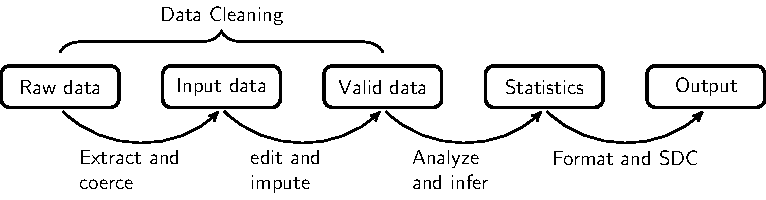
\includegraphics[width=\textwidth]{fig/valuechain.pdf}
\caption{Part of a statistical value chain, showing five different levels of 
statistical value going from raw data to statistical product.}
\label{fig:valuechain}
\end{figure}
A nice trait of the schema in Figure~\ref{fig:valuechain} is that it naturally
introduces activities that are typically categorized as `data cleaning' into
the statistical production process. From the left we start with raw data.  This
must be worked up to satisfy (enough) technical standards so it can serve as input
for consistency checks, data correction and imputation procedures.  Once this
has been achieved, the data may be considered valid (enough) for the production
of statistical parameters. These must then still be formatted to be ready for
deployment as output. 



More generally, a statistical production process is designed by viewing
input, output and a number of intermediate states as statisitical products.
\begin{terminology}{Statistical product}
A state of data that is guaranteed to satisfy a predifined set of quality
demands. 
\end{terminology}
Thus each state, represented by a rectangle in Figure~\ref{fig:valuechain} is
fixed by specifying precisely when a data set is allowed to be called `raw', or
`valid' and so on. Physically, each state may be represented by a table in a
data base, a set of files, or any other way data can be represented. A
description should be accurate enough to understand the contents of a data set
as well as the limits of its usability. To describe usability, the five quality
aspects defined in the Eurpean Quality Assurance Framework (QAF): relevance,
accuracy, timeliness, accessibility and comparability serve as a guide of
things to describe. For example, a good description of the file format falls
under accessibility while an accurate description of logical restrictions that
the data satisfy (like `Age is nonnegative') falls under 'accuracy and
reliability'.


\begin{terminology}{The five quality aspects of data}
  In the European Quality Assurance Framework, the following five quality 
  dimensions are defined.
  \begin{itemize}
    \item\textbf{Relevance.} The degree to which the statistical product meets
    user needs in both coverage
    and content.
    \item\textbf{Accuracy \& Reliability.} Accuracy is the proximity between an estimate
    and the unknown true value. Reliability is the closeness of early estimates to
    subsequent estimated values.
    \item\textbf{Timeliness and Punctuality.} Timeliness refers to the time gap between
    publication and the reference period. Punctuality refers to the gap between
    planned and actual publication dates.
    \item\textbf{Accessibility and Clarity.} Accessibility is the ease with which users are
    able to access the data, also reflecting the format in which the data are
    available and the availability of supporting information. Clarity refers to the
    quality and sufficiency of the metadata, illustrations and accompanying advice.
    \item\textbf{Comparability and Coherence.} Comparability is the degree to which data
    can be compared over time and domain. Coherence is the degree to which data
    that are derived from different sources or methods, but refer to the same
    topic, are similar.
  \end{itemize}
\end{terminology}

Having solid descriptions of each state are an important step of making data
usable for other production processes or incidental analyses.  It makes
different statistical production chains composable by using the output of one
chain as input for another.  The definition of statistical products allows one
to systematically disentangle a complex set of activities going from input to
output into manageable chunks of well-defined tasks with clear beginnings and
clear ends. This allows one to design the process going from say `input data'
to `valid data' independent from the other steps in the chain.  If two
statistical production processes have similar intermediate states, there is a
chance that tooling and methodology might be shared between them, thus
enhancing standardisation, which in turn should improve comparability between
statistics and overall efficiency.

One generally distinguishes two approaches in designing statistical production
chains. The first and traditional way is called \emph{output-driven} design.
Here, one first investigates the need of end-users and based on that, describes
the output state with all quality aspects. For example, the output may be an
interactive dashboard that gives a coherent view on the state of a certain
economic sector. Given this description, one can then describe what statistics
should be available, and with what quality.  Knowing this, one can describe the
necessary microdata and it's quality necessary to produce the statistics. This
process continues until the necessary raw data is defined. 

The second and more recent approach to Statistical Value Chain design is called
the \emph{data-driven} approach. The motivation is usually the availability of
a new type of data source that is potentially interesting for the production of
official statistics. Either by creating an opportunity for new output or for
replacing or augmenting an existing data source. In this case, the 'design'
process is more informal and proceeds iteratively, starting with investigating
the usability of the data. Once usability is established, more iterations are
necessary to actually bring the new process into production.

We conclude this section by describing the five data states of
Figure~\ref{fig:valuechain} in some more detail.

\subsection*{Raw data}
With raw data we mean the data as it arrives at the place where it is to be
processed. The state of such data may of vary enormously depending on the data
source.  Raw data is often characterized by limited amount of control over how
the data was collected, as is the case with administrative data. However, it is
possible to describe the state of the data as it arrives and perhaps to create
agreements with data suppliers about data form and quality. In any case,
a version of the raw data is to be stored as-is to ensure reproducibility.

\begin{terminology}{Raw data}
Raw data is `data as it arrives'. We only demand that it is adequately
described so further processing can take place.
\end{terminology}

The first production step, consist of making the data readily accessible and
understandable. After the first processing step, we demand that each value in
the data can be identified with the real-world object they represent (person,
company, something else), for each value it is known what variable it
represents (age, income, ...), and the value is stored in the appropriate
technical format (number, string).

Depending on the technical raw data format, the activities necessary to achieve
the desired technical format typically include file conversion, string
normalization, and standardization and conversion of numerical values. Joining
the data against a backbone population register of known statistical objects,
possibly using procedures that can handle inexact matches of keys is also
considered a part of such a procedure. 


\subsection*{Input data}
Input data are data where each value is stored in the correct type and
identified with the variable it represents and the statistical entity it
pertains to. In many cases such a dataset can be represented in tabular format,
rows representing entities, columns representing variables.  In the R community
this has come to be known as `tidy' data \citep{wickham2014tidy}.  Here, do not
force a particular data format. Many data can be usefully represented in the
form of a tree or graph (e.g. web pages, XML structures). As long as all the
elements are readily identified and of the correct format, it can serve as
Input data.

\begin{terminology}{Input data}
Input data satisfies the following demands.
\begin{itemize}
\item Each unit in the data is identified with a unit in the population register.
\item Each unit occurs only once in the data.
\item Each value is stored in the correct type (a data type defines the values
      that a variable can assume).
\item Each value is identified with a single population unit and a single attribute of that unit.
\end{itemize}
\end{terminology}
A rule of thumb for input data is that it can be easily imported into an
appropriate tool. For example by reading it from a data base, or a
well-described textual format, in a single line of script.


Once a dataset is at the level of input data, the treatment of missing values,
implausible values, and implausible value combinations must take place. This
process is commonly referred to as data editing and imputation. It differs from
the previous steps in that it focuses on the consistency of data with respect
to domain knowledge. Such domain knowledge domain knowledge can often be
expressed as a set of rules, such as \code{age >= 0}, or \code{mean(profit) >
0}, or \code{if ( age < 15 ) has\_job = FALSE}. We will have a further look
into such rules in Chapter~\ref{sect:datavalidation}.

%%%%%%%%%%%%%%%%%%%%%%%%%%%%%%%%%%%%%%%%%%%%%%%%%%%%%%%%%%%%%%%%%%%%%%%%%%%%%%%
\subsection*{Valid data}
Data are valid once they are trusted to faithfully represent the variables and
objects they represent. Making sure that data satisfies the domain knowledge
expressed in the form of a set of validation rules is one reproducible way of
doing so. Often this is complemented by some form of expert review, for example
based on various visualizations, or reviewing of aggregate values by domain
experts.

\begin{terminology}{Valid data}
Data is `valid' when it contains no invalid values, is free of internal
contradictions, and does not conflict common domain knowledge.
\end{terminology}

Once data is deemed valid, the statistics can be produced by known modeling and
inference techniques. Depending on the preceding data cleaning process, these
techniques may need those procedures into account. For example when estimating
variance after certain imputation procedures.


%%%%%%%%%%%%%%%%%%%%%%%%%%%%%%%%%%%%%%%%%%%%%%%%%%%%%%%%%%%%%%%%%%%%%%%%%%%%%%%
\subsection*{Statistics}
Statistics are simply estimates of the output variables of interest. Often these
are simple aggregates (totals, means) but in principle they can consist of more
complex parameters such as regression model coefficients, or a trained 
machine learning model. 

\begin{terminology}{Statistics}
A statistic is an estimate of a population property based on valid data.
\end{terminology}

Once statistics are computed, they need to be formatted to be transferred to
other organizations or for presentation.

%%%%%%%%%%%%%%%%%%%%%%%%%%%%%%%%%%%%%%%%%%%%%%%%%%%%%%%%%%%%%%%%%%%%%%%%%%%%%%%
\subsection*{Output}
Creating output begins where the analysis stops. Output is created by taking
the statistics and preparing them for dissemination. This may involve technical
formatting, for example to make numbers available through a (web) API or layout
formatting, for example by preparing a report or visualization. In the case of
technical formatting, a technical validation step may again be necessary, for
example by checking the output format against some (json or XML) schema. In
general, the output of one institute or department is raw data for another.
\begin{terminology}{Output}
Data formatted for dissemination.
\end{terminology}

\newpage{}
\section{Exercises}
\label{sect:exsvc}
\begin{enumerate}
  \item Explain where in the value chain of Figure~\ref{fig:valuechain} the following 
  activities take place. Sometimes multiple options are possible. Explain why.
  \begin{enumerate}
    \item Formatting a date-time variable to ISO8601 format.
    \item Estimate the covariance between unemployment rate and age.
    \item Join survey data with a survey reference frame, using unique identifiers
          (such as social security number) so all elements in the survey data can be
          identified.
    \item Join administrative data with a reference frame, using approximate record linkage,
          based on approximate matches in name-addres data.
    \item Clean up a text variable that contains values such as \code{"M"}, \code{"Man"},
          \code{"Fem"}, and \code{"woman"} and replace them with valid codes from a code
          list, like \code{"male"} \code{"female"}, \code{"other/non-binary"}.
  \end{enumerate}
  \item Discuss advantages and disadvantages of the data-driven versus the
        output-driven approach to designing statistical production systems.
\end{enumerate}

\hfill{}Check your answers on page~\pageref{sect:anssvc}.
